\chapter{Experimental setup}\label{ch:experimental-setup}

In this chapter we will introduce our dataset, the structure of the model, our metrics and evaluation approach to be able to compare different inpainting transformer based models.

\section{Data}

We use the MVTec AD dataset that we previously mentioned in section \ref{sec:relwork:anomaly-detection}. This dataset is also used by other researchers \cite{pirnay_inpainting_2021, bergmann_improving_2019, zavrtanik_reconstruction_2021} to compare the performance of methods for anomaly detection. The dataset focuses on industrial anomalies, which can be used for both the detection and the segmentation or localisation of anomalies. The dataset contains 15 different images, categorised into textures and objects. Some of the images are photos taken in 1 place and orientation, while others contain different rotations or positioning. This variation makes it  The images with defects in the dataset are labeled by anomaly type and  segmentation maps are provided for localisation of the anomalies in those images.

\begin{figure}[h!]
\caption{An example of a screw, toothbrush and transistor that are defective.}
\centering
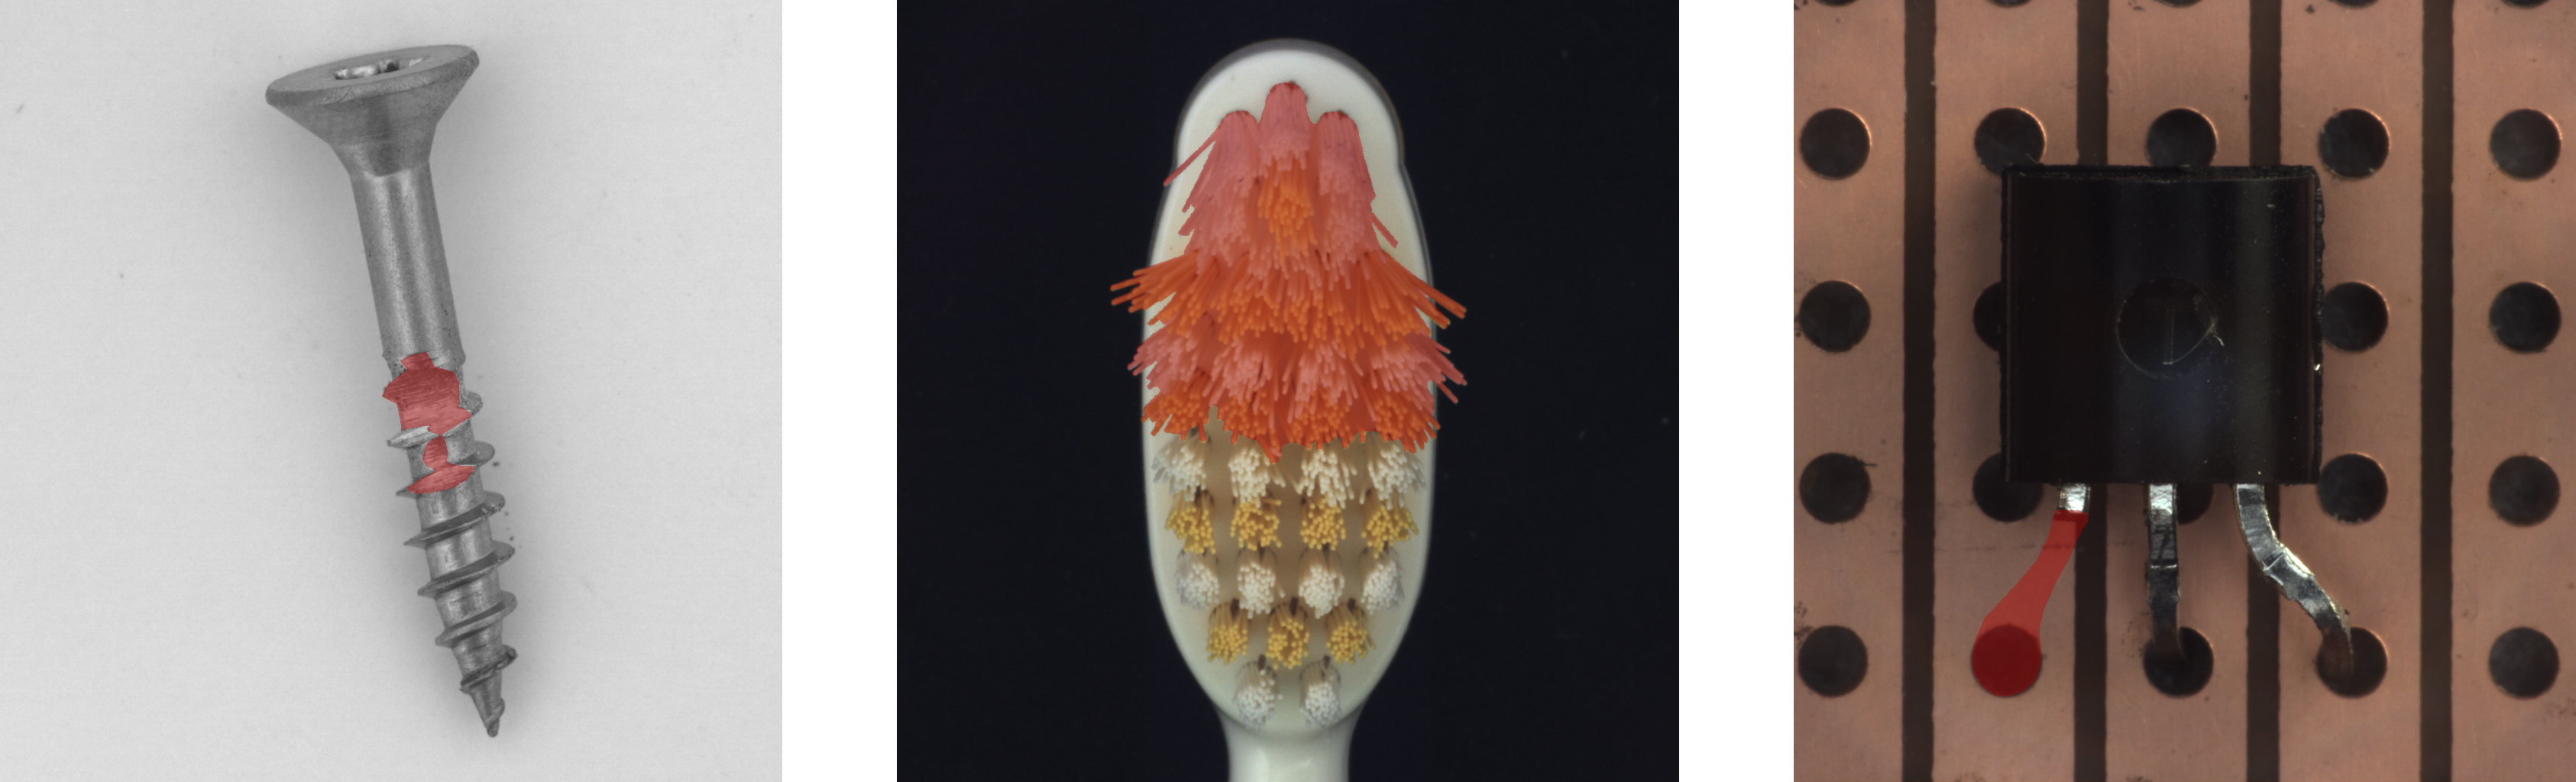
\includegraphics[width=\textwidth]{imgs/mvtec-example-objects.jpg}
\label{fig:experimental-setup:objects-example}
\end{figure}

\begin{figure}[h!]
\caption{An example of a piece of leather, tile and grid that are defective.}
\centering
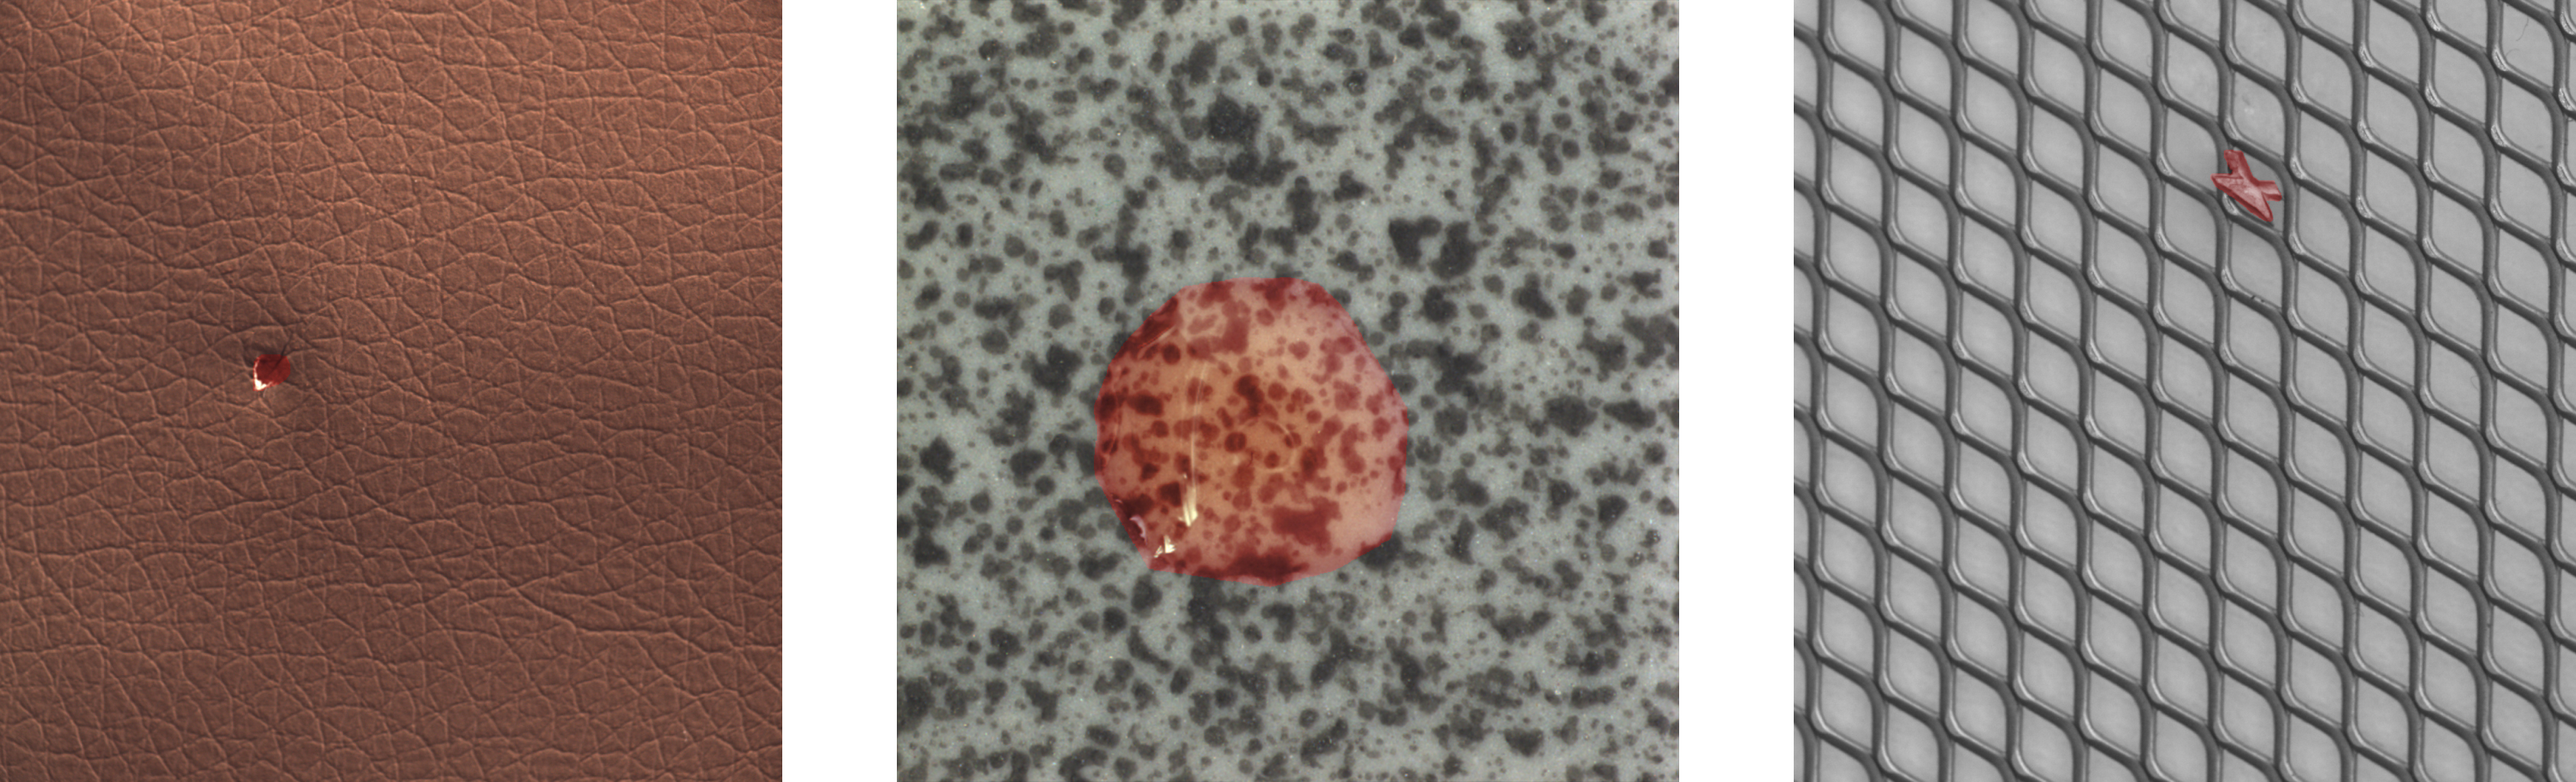
\includegraphics[width=\textwidth]{imgs/mvtec-example-textures.jpg}
\label{fig:experimental-setup:textures-example}
\end{figure}

In figure \ref{fig:experimental-setup:objects-example} we see three different object-type images with defects. Compared to figure \ref{fig:experimental-setup:textures-example} where we have examples of textures. These different types of images allow us to test our model to do both detailed texture synthesis and structure inpainting. In the case of anomaly detection the defects on the textured images are smaller and require finer reconstruction of the texture details when compared to the larger objects where the anomalies usually consist of larger deformations or missing elements.

\section{Model}
\label{sec:experimental-setup:model}

Our inpainting transformer model is directly based on the inpainting transformer by Pirnay et al. \cite{pirnay_inpainting_2021}. For completeness we will introduce the patch embeddings used for the inpainting problem and give an overview of the model architecture.

\subsection{Patch embeddings}

The model uses a patch based approach to create full reconstructions of images. Each image is split into patches of which one is covered. The model then learns to inpaint that patch based on the surrounding patches. The creation of the patches is similar to the approach discussed in section \ref{sec:prelim:transformers:vision}. An overview of these step can be found in figure \ref{fig:experimental-setup:intra-overview}a.

We start by defining our images as $x \in \mathbb{R}^{H \times W \times C}$ where $H$ is the height, $W$ the width and $C$ the number of channels. We create square patches of the size $(P, P)$. This means that we can split each image into a grid of $M \times N$ patches where $M = \frac{W}{P}$ and $N = \frac{H}{P}$:
%
\begin{align}
    x_p \in \mathbb{R}^{(M \times N) \times (P^2 \; \cdot \; C)}\\
    x_p^{(i,j)} \in \mathbb{R}^{P^2 \; \cdot \; C}
\end{align}
%
with $(i, j)$ denoting the location of the patch within in the image.

We then want a square window of patches of length $L$ that is smaller than the image. From this window we can the pick any patch that should be inpainted based on the other patches in the same window. In \cite{pirnay_inpainting_2021} they formulate this inpainting problem as follows:

\begin{quote}
Let $(x_p^{(i,j)})_{(i,j) \;\in\; S}$ be a square subgrid of patches defined by some index set $S = {r,...,r+L-1} \times {s,...,s+L-1}$. Here $L$ is the side length of the window, and $(r,s)$ is the grid position of the upper left patch in the window. If $(t, u) \;\in\; S$ is the position of some patch, the formal task to inpaint $(t,u)$ is to approximate the patch $x_p^{(t,u)}$ using only the content and the positions of all other patches $(x_p^{(i,j)})_{(i,j) \;\in\; S \;\setminus\; {(t,u)}}$ in the window.
\end{quote}

This means that for the transformers to able to determine the position of the patches we need to include information of the position of a patch $x_p^{(i,j)}$. For this we calculate a one dimensional value:
%
\begin{align}
f(i,j) = (i-1) \;\cdot\; N + j 
\end{align}
%
As a last step we need to reshape this patch window into an input sequence for our transformer-based model. We do this by creating a mapping in some latent space of dimension D. Which means that for every patch $(x_p^{(i,j)})_{(i,j) \;\in\; S \;\setminus\; {(t,u)}}$ we create and embedding $y^(i,j)$ and for the patch we ant to inpaint we add one single embedding $x_{inpaint} \in \mathbb{R}^D$ to the position embedding.
%
\begin{align}
y^(i,j) = x_p^{(i,j)}E + posemb(f(i, j)) \in \mathbb{R}^D\\
z = x_{inpaint} + posemb(f(t, u)) \in \mathbb{R}^D
\end{align}
%
where $E \in \mathbb{R}^{(K^2 \;\cdot\; C) \times D}$ and $posemb$ is a standard learnable one-dimensional position embedding.

This means that the final input sequence for the model is then formed by $z$ and $y^{yi, j}$ for each $(i, j) \;\in\; S \setminus {(t,u)}$.

\begin{figure}[ht!]
\caption{An overview of the inpainting transformer steps by Pirnay et al. \cite{pirnay_inpainting_2021}}
\centering
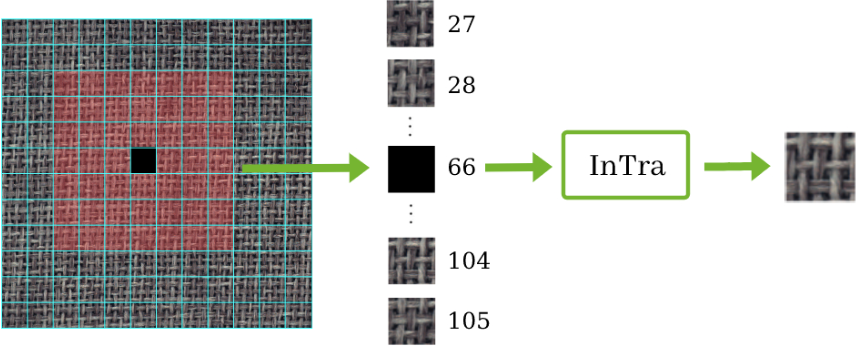
\includegraphics[width=\textwidth]{imgs/intra-overview.png}
\label{fig:experimental-setup:intra-overview}
\end{figure}

\subsection{Architecture}

The architecture for our inpainting model uses $n$ blocks of the transformer encoders that are stacked.
It consists of an attention function and a fully-connected feed-forward network. This follows the approach of the Vision Transformer discussed in section \ref{sec:prelim:transformers:vision}. The structure of this model is visualised in figure \ref{fig:experimental-setup:model-structure}.

\begin{figure}[ht!]
\caption{The structure of our inpainting model}
\centering
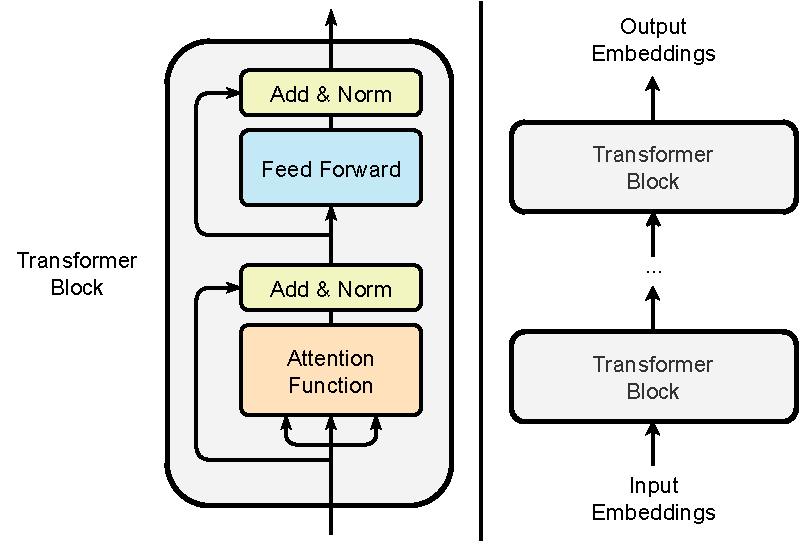
\includegraphics[width=\textwidth]{imgs/model-structure.pdf}
\label{fig:experimental-setup:model-structure}
\end{figure}

We create two different versions of our model. One of these versions uses the original multi-head self-attention (MSA) from \cite{vaswani_attention_2017} that we discussed in section \ref{sec:prelim:transformers:vanilla}. The second version uses the linearised multi-head self-attention (LMSA) from \cite{katharopoulos_transformers_2020} that we discussed in section \ref{sec:prelim:transformers:linear}.

This differs from the original InTra model in two places: we do not add residual connections between layers and we do not use multi-head feature self-attention. This allows us to directly compare the two attention functions for our inpainting task.

\section{Loss function}
\label{sec:experimental-setup:loss}

To be able to quantify the performance of our models during training we require metrics that are suitable for the inpainting task that we are performing. This means that we need a loss function that takes into account that our dataset contains both textures and objects. For this we use a combination of structural similarity, gradient magnitude similarity and a pixel-wise L2 loss.

Since we try to recreate the model from \cite{pirnay_inpainting_2021} we also use a similar loss function. Which is equal to the one used in \cite{zavrtanik_reconstruction_2021}.

Our loss function L consists of three parts. The first part is a pixel-wise $L_2$ loss. This does not take into account perceptual differences, since it assumes that all pixels in the images are independent. Therefore we also use the structured similarity index (SSIM) \cite{bergmann_improving_2019} and the multi-scale gradient magnitude similarity (MSGMS) \cite{xue_gradient_2014, zhang_gradient_2017}.

The SSIM is a metric that looks at dependencies between regions of an images by including luminance, contrast and structural information. This means that it assumes that our model is able to find those structures. MSGMS is similar in that it looks at local image quality but does not focus on those structures.
\\
Before we determine the full loss function we first formulate these three base parts given our original patch $P$ and the reconstruction $\hat{P}$ for that patch.

\begin{align}
L_{SSIM}(P, P) = \frac{1}{N_p} \sum_{x=1}^{W}\sum_{y=1}^{H}{} {1 - SSIM_{(x,y)}(P_l, \hat{P}_l)}
\end{align}

where $N_p$ is the number of pixels of the patch $P$. The $SSIM_(x,y)$ is the SSIM result for the two pixel in the patch and the reconstruction with $(x,y)$ being the center.

\begin{align}
L_{MSGMS}(P, P) = \frac{1}{3} \sum_{l=1}^{3} \frac{1}{N_l} \sum_{x=1}^{W_l}\sum_{y=1}^{H_l}{} {1 - GMS_{(x,y)}(P_l, \hat{P}_l)}
\end{align}

where $N_l$ is the number of scales. $P_l$ and $\hat{P}_l$ the scaled version of the patches and $GMS_{(x,y)}(P_l, \hat{P}_l)$ gives the GMS map of those scaled patches at the pixel location $(x,y)$.

\unsure{Maybe extend the bit explaining the GMS in more detail? Possibly in the preliminaries in image similarity section}

We can then define our complete loss function as 

\begin{align}
L(P, \hat{P}) = L_2(P, \hat{P}) + \alpha \; L_{MSGMS}(P, \hat{P}) + \beta \; L_{SSIM}(P, \hat{P})
\end{align}

with $\alpha$ and $\beta$ being loss weights for the MSGMS and SSIM losses.

\section{Anomaly detection}\label{sec:methods-setup-ad}

To be able to use our model for anomaly detection we need to generate a complete reconstruction of some original input image. This reconstruction can then be used to create a anomaly map where we can locate any anomalies.

\subsection{Reconstruction}

The reconstruction $\hat{x}$ of the image $x \in \mathbb{R}^{H \times W \times C}$ requires us to split the image into the same number of $M \times N$ patches as the images we used to train our models.
We can then create a reconstruction by selecting a window with size $L x L$ per patch $x_p^{(t,u)}$ to create a reconstruction of that section of the image.

The ideal window for each patch is the window location where the $(t,u)$ is in the center. Since we want to create a reconstruction of the full image this is not possible for the patches closer to the sides of the image itself. Therefore we want to calculate an appropriate patch window with patch $x_p^{(r,s)}$ in the upper-left corner.

%
\begin{align}
pad(x) = max(1, x - \lfloor \frac{L}{2} \rfloor)\\
r = pad(t) - max(0, pad(t) + L - N - 1)\\
s = pad(u) - max(0, pad(u) + L - M - 1)
\end{align}
%

Reconstructing the image can now be done by using the calculated windows for each patch. This gives us the fully reconstructed image $\hat{x}$.

\subsection{Anomaly map}

With both our original image $x$ and the reconstruction $\hat{x}$ we can create an anomaly map that we can use to detect and locate anomalies in $x$. For this we use similar multi-scale gradient magnitude similarity calculations that we also used for our loss function in section \ref{sec:experimental-setup:loss}.

Instead of a single value we want a complete map thus we adapt the calculation slighty to create a per-pixel average of the GMS maps at different scales. Similar to the approach in \cite{pirnay_inpainting_2021, zavrtanik_reconstruction_2021}.

\begin{align}
MSGMS(I, \hat{I}) = \frac{1}{3} \sum_{l=1}^{3} {GMS(I_l, \hat{I}_l)}
\end{align}

Since anomalies are usually located in larger connected regions of an image we can aggregate the error of the reconstruction over a larger space by post-processing the MSGMS map using a mean-filter convolution. This smoothing removes the detection when high values are present in the MSGMS map in small regions of the image. These values are more likely to be failed reconstructions or background noise.

\begin{align}
diff(I, \hat{I}) = 1_{H \times W} - (MSGMS(I, \hat{I}) \ast mean)
\end{align}

\todo{anomap}



% The anomaly score map is obtained by first calculating the GMS map considering the input and the reconstructed image over multiple scales. In particular, for each scale l a scaled GMS map is computed by (4) from the input Il and reconstructed image Irl downsampled to the scale l, using the same down-sampling procedure as when computing the MSGMS loss during training. GMS(Il , Irl ) is then upsampled to the original resolution. A multiscale GMS map MSGMS(I, Ir ) is then computed as the per-pixel average of the scaled GMS maps. Anomalies tend to occupy larger spatially connected regions, therefore the reconstruction error can be aggregated over a larger region for a more accurate anomaly detection. The MSGMS map is thus postprocessed by a mean-filter convolution and subtracted from a matrix of ones to generate the anomaly map G(I, Ir ) ∈ [0, 1]H×W


\section{Training}

Using the building blocks given in the previous sections we train 2 models per image in the MVTecAD dataset. This way we can compare the result of the different MSA and MLSA attention functions.

The parameters we used during training are mostly the same as those in \cite{pirnay_inpainting_2021}.

For training we use the images without anomalies from MVTec AD. Each set of training data contains a different number of images and no predefined validation set. This is why randomly take 10\% or 20 images from the training data to be able to check the patches that our models generate.

The rest of the training data is used to extract 600 random patch windows per epoch per images. This increases the amount of training data and shuffles the input.

Other parameters define the size and number of patches: patch size $P$, window size $L$ and the size of the images $W$ and $H$. Since all images in MVTec AD are square this means that $W \;=\; H$. These parameters are set to $P = 16$ and $L = 7$. The image sizes differ per image: $256 \times 256$, $320 \times 320$, $512 \times 512$. These were chosen by Pirnay et al. as small as possible without removing details from the patches.

We use a latent dimension of $D = 512$ for our training runs. Both the MSA and MLSA models consist of 13 transformer blocks that have 8 attention heads. This gives us $41,374,976$ trainable parameters. The individual loss weights are set to $\alpha = \beta = 0.01$ and all models are trained with the same Adam optimizer with the learning rate set to $0.001$. The batch size is set to $256$ and all probabilities for dropout are set to $0$.

\todo{Stuff about the kernel size for the msgms map}

To be able to find differences in the training time and to make sure our models fully converge we train our models for a maximum number of $20000$ epochs, which is virtually unlimited since we combine this with early stopping of 150 epochs. The best model is then chosen based on the lowest validation loss.

Each model is trained by submitting a job on a SLURM cluster. The jobs are assigned 4 CPU cores, 1 GPU and maximum 16 GB of memory. The nodes in the cluster are outfitted with 2x Intel Xeon Silver 4214, 8x NVIDIA GeForce RTX 2080 Ti and 128GB of memory.

\section{Evaluation}

To be able to compare two different transformer models we will use the ROC AUC, which is standard for visual anomaly tasks \cite{pirnay_inpainting_2021, zavrtanik_reconstruction_2021, schlegl_unsupervised_2017, li_cutpaste_2021, tsai_autoencoder-based_2021, xie_semisupervised_2021, bergmann_mvtec_2019}.

For this we will use the anomaly map $anomap(x)$ we obtained from the images in section \ref{sec:methods-setup-ad}.

We want to evaluate both the anomaly detection on the image-level and the anomaly segmentation on the pixel-level. For the last task we can directly use the anomaly map. For the image-level detection we take the maximum pixel value from the anomaly map as a single anomaly score for the whole image.